\begin{frame}
\frametitle{Ao final dessa aula, você será capaz de:}
\begin{itemize}
 \item Compreender o que é um projeto
 \item Classificar um projeto como bem sucedido ou não
 \item Compreender o que faz um projeto bem sucedido
 \item Compreender a complexidade do gerenciamento
 \item Quem são as partes envolvidas em um projeto
 \item Guia PMBok
\end{itemize}
\end{frame}

\section{O que é Projeto?}

\begin{frame}
\frametitle{Contexto}
\begin{itemize}
 \item Cerca de 12 trilhões de dólares são hoje empregados em projetos
 %\pause
 \item  25 \% da economia mundial empregando 20 milhões de profissionais
 %\pause
 \item Tom Peters afirmou em 1999 que em 20 anos todo o trabalho será desenvolvido por meio de projetos
 %\pause
 \item O gerenciamento de projetos não propõe nada revolucionário e novo
\end{itemize}
\end{frame}

\begin{frame}
 \frametitle{Contexto}
 \begin{itemize}
  \item A Competitividade impulsiona o gerenciamento de projetos
  %\pause
  \item É preciso que se tenha habilidade em gerenciar aquilo que se conhece muito pouco, ou até mesmo aquilo que não se conhece nada
  %\pause
  \item  Os projetos atingem todos os níveis de uma organização
  %\pause
  \item Podem levar 1 dia ou vários anos
 \end{itemize}
\end{frame}

\begin{frame}
 \frametitle{Projeto}
 \begin{figure}
  \centering
  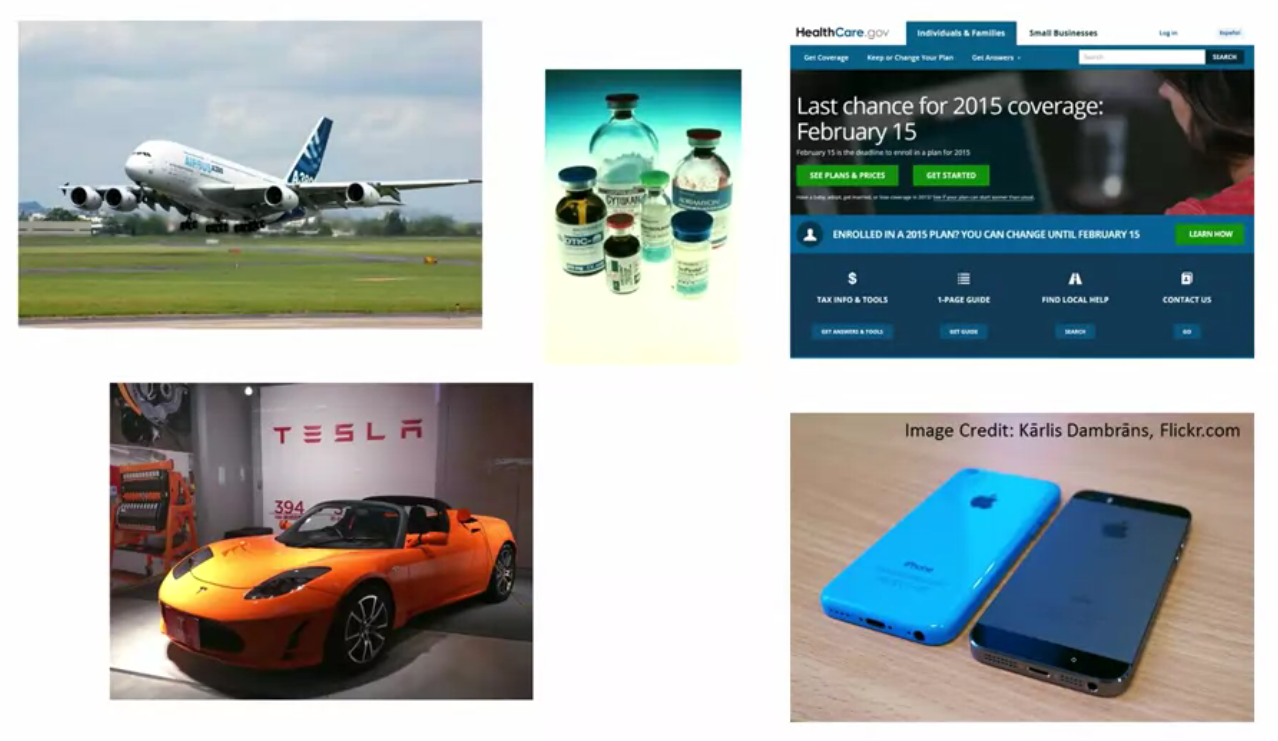
\includegraphics[width = \textwidth]{figs/fig_proj1.png}
 \end{figure}
\footnote{Fonte: Fundamentals of Project Planning and Management - Coursera}
\end{frame}

\begin{frame}
 \frametitle{Projeto}
 \begin{figure}
  \centering
  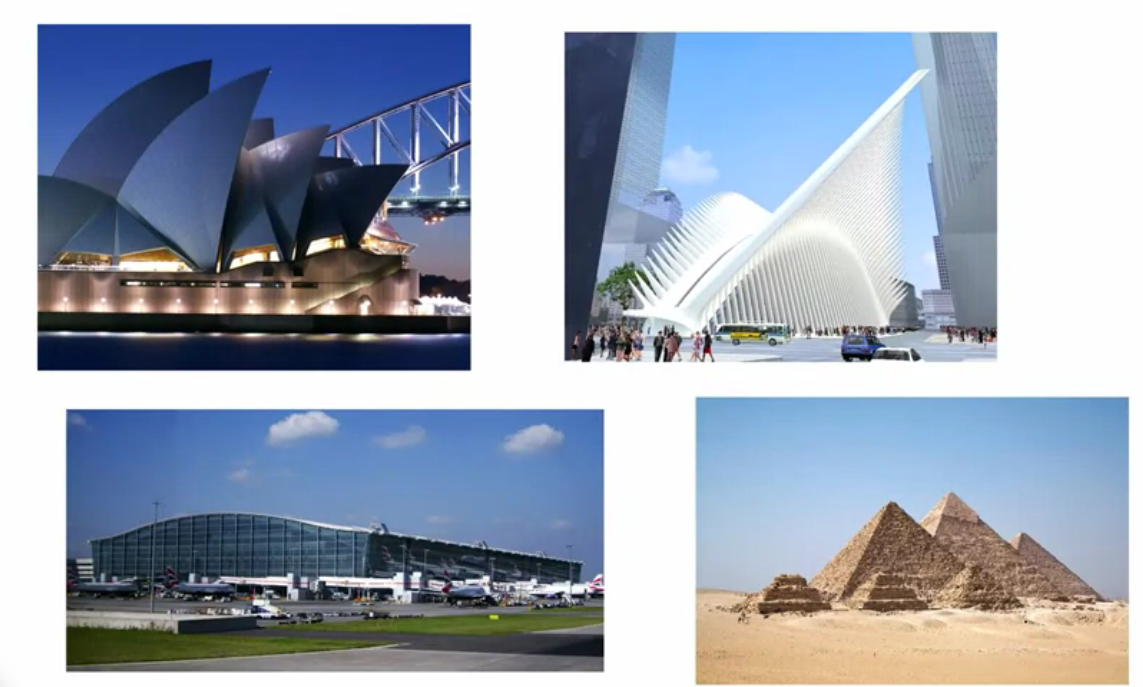
\includegraphics[width = \textwidth]{figs/fig_proj2.png}
 \end{figure}
\footnote{Fonte: Fundamentals of Project Planning and Management - Coursera}
\end{frame}

\begin{frame}
 \frametitle{Projeto}
 \begin{figure}
  \centering
  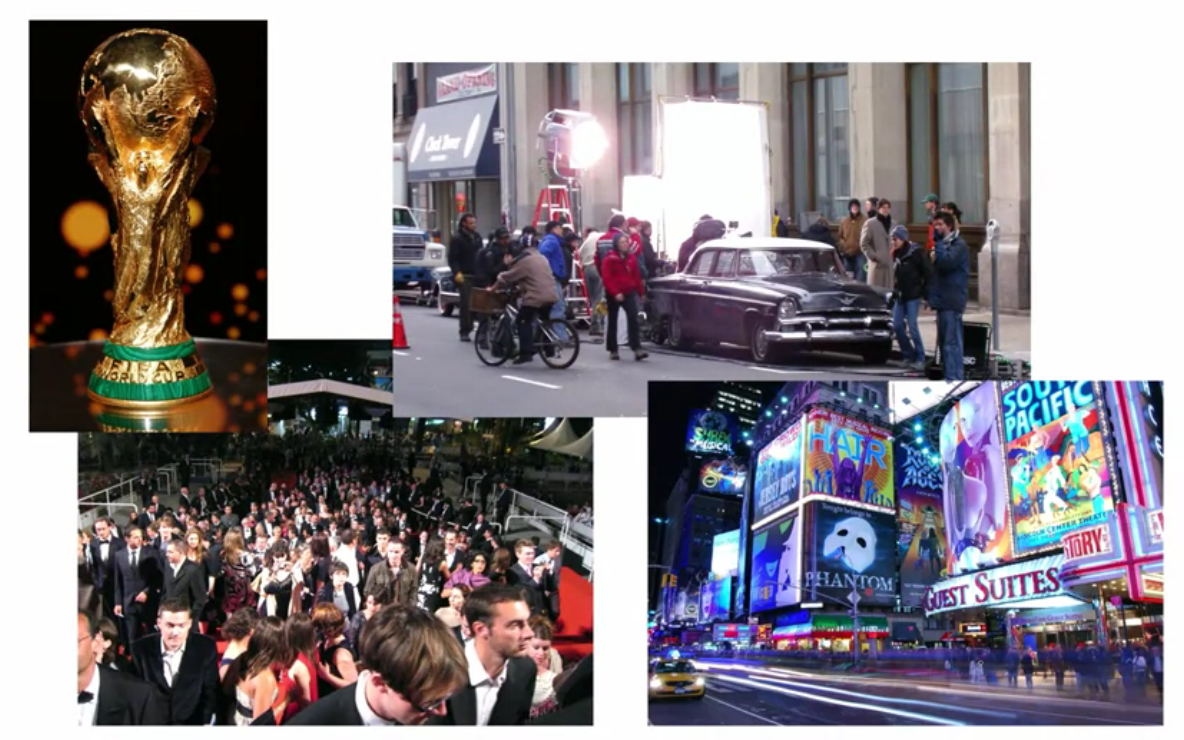
\includegraphics[width = \textwidth]{figs/fig_proj3.png}
 \end{figure}
\footnote{Fonte: Fundamentals of Project Planning and Management - Coursera}
\end{frame}


\begin{frame}
 \frametitle{O que é um Projeto?}
 \begin{itemize}
  \item Definição de Projeto:
  \begin{itemize}
   \item é um empreendimento \textbf{não repetitivo}
    %\pause
   \item caracterizado por uma sequência clara e lógica de eventos com \textbf{início, meio e fim definidos}
   %\pause
   \item se destina a atingir um \textbf{objetivo claro e definido}
   %\pause
   \item conduzido por \textbf{pessoas}
   %\pause
   \item  \textbf{parâmetros pré-definidos} de tempo, custo, recursos envolvidos e qualidade
  \end{itemize}
 \end{itemize}
\end{frame}

\begin{frame}
 \frametitle{Projeto - Definições formais}
 \begin{block}{Harvard Business Review}
  \textit{"A \textbf{unique} set of activities meant to produce a defined outcome within an established \textbf{time frame} using specific allocation of resources"}	
 \end{block}

 \begin{block}{Project Management Institute}
  \textit{"A project is a \textbf{temporary} endeavor undertaken to create a \textbf{unique} product or service"}
 \end{block}
\end{frame}

\begin{frame}
 \frametitle{Características de Projetos}
 \begin{itemize}
  \item Temporariedade
  \begin{itemize}
   \item todo projeto possui um início e fim definidos, ou seja, é um evento com \textbf{duração finita}, determinada em seu objetivo.
  \end{itemize}
  %\pause
  \item Individualidade
  \begin{itemize}
   \item Significa realizar algo que não tenha sido realizado antes. 
    \item Como o \textbf{produto} de cada projeto é \textbf{único}, suas características precisam ser elaboradas de maneira progressiva
    de modo a garantirem as especificações do produto ou serviço a ser desenvolvido
  \end{itemize}
 \end{itemize}
  \end{frame}

  \begin{frame}
   \frametitle{Características de Projetos}
   \begin{itemize}
    \item A partir do entendimento de temporariedade e Individualidade, então é possível descrever as demais
    %\pause
    \begin{itemize}
     \item Empreendimento não repetitivo – evento que não faz parte da rotina da empresa
     %\pause
     \item Sequência clara e lógica – atividades encadeadas logicamente de modo a permitir que, durante a execução, o acompanhamento e controle
     %\pause
     \item Início, meio e fim – ter uma característica temporal; ter início-meio-fim não significa ser longo ou curto em duração	
    \end{itemize}
   \end{itemize}
  \end{frame}
  
  
  \begin{frame}
   \frametitle{Características de Projetos}
   \begin{itemize}
    \item Elaboração progressiva é a característica de projeto que integra os conceitos de temporário e único
    %\pause
    \item Elaboração progressiva significa desenvolver em etapas e continuar por incrementos
    \begin{itemize}
    %\pause
     \item Como o produto de cada projeto é único, as características peculiares que o distinguem devem ser progressivamente elaboradas. 
      %\pause
     \item Estas características que distinguem os produtos a serem construídos são definidas de forma genérica no início do  projeto, e se tornam mais explícitas e detalhadas assim que a equipe adquire uma melhor e mais completa percepção do produto ou serviço.
    \end{itemize}
   \end{itemize}
  \end{frame}
  
\begin{frame}
 \frametitle{O que não é Projeto}
  \begin{figure}
  \centering
  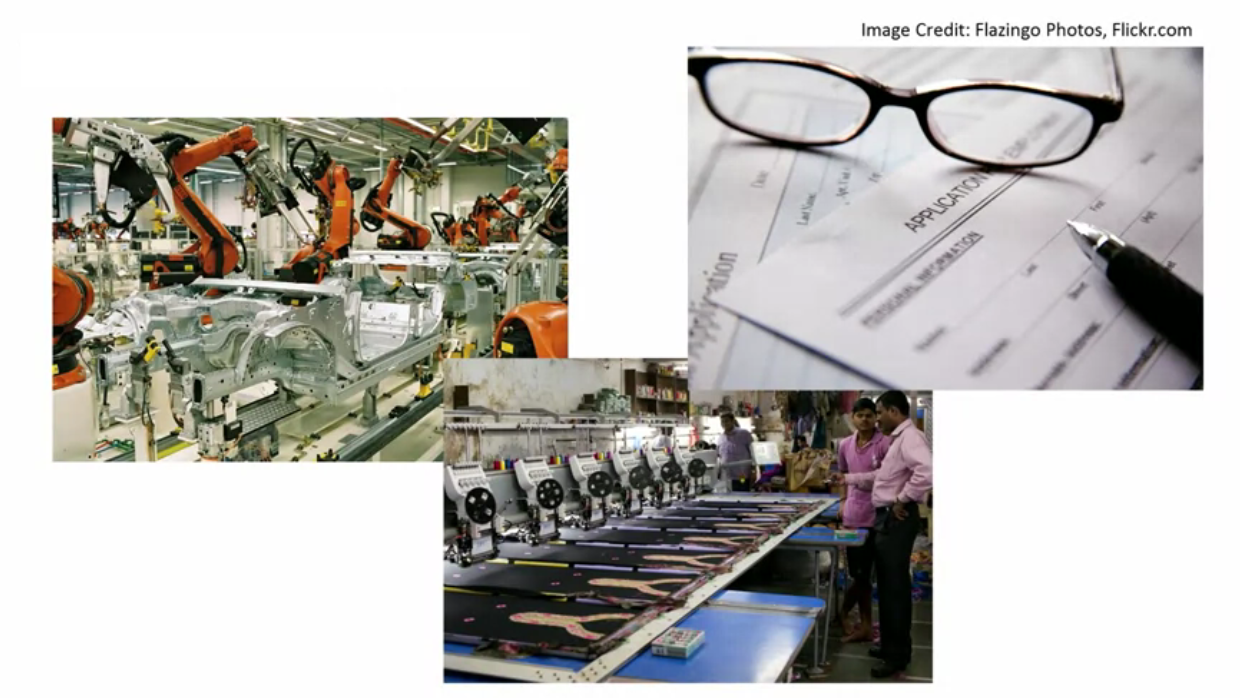
\includegraphics[width = \textwidth]{figs/fig_proj4.png}
 \end{figure}
\footnote{Fonte: Fundamentals of Project Planning and Management - Coursera}
\end{frame}

\begin{frame}
 \frametitle{Por que compreender o que é ou não projeto?}
  \begin{itemize}
  \item Compreender o que é um projeto auxilia a planejá-lo e executá-lo melhor com as ferramentas adequadas
  \item Projetos e Processos:
  \begin{itemize}
   \item Objetivos Diferentes
   \item Diferentes critérios de Sucesso
  \end{itemize}
  \item Produtos não são únicos em serem únicos
 \end{itemize}
\end{frame}


\section{Gerenciamento de Projetos}

  \begin{frame}
   \frametitle{Gerenciamento de Projetos}
\begin{block}{Gerenciamento Geral}
  O gerenciamento geral inclui o planejamento, a organização, a formação de pessoal, a
execução e o controle de operações de uma empresa existente.
\end{block}
  \end{frame}
  
  \begin{frame}
   \frametitle{Gerenciamento de Projetos}
   \begin{block}{Gerenciamento por Projetos}
    É importante observar que muitos processos dentro do gerenciamento de
projetos são iterativos devido à existência, e necessidade, de uma elaboração
progressiva em um projeto durante todo o ciclo de vida do projeto.
   \end{block}
  \end{frame}


\section{Definindo o Projeto e Objetivos}

\begin{frame}
 \frametitle{Diferenciando Projetos, Subprojetos, Programas e Portfólios}
 \begin{itemize}
  \item Subprojetos
  \begin{itemize}
   \item Os subprojetos são responsáveis por uma \textbf{pequena parte} do projeto total ou por \textbf{fases extremamente específicas} do
   projeto e podem, na maioria das vezes, ser terceirizadas ou desenvolvidas por grupos isolados
  \end{itemize}
  \item Programa
  \begin{itemize}
   \item Grupo de \textbf{projetos relacionados} que são \textbf{gerenciados e coordenados} de \textbf{modo integrado}, obtendo os benefícios e controles que
   não existem ao gerenciá-los individualmente
  \end{itemize}
 \end{itemize}
\end{frame}

\begin{frame}
 \frametitle{Diferenciando Projetos, Subprojetos, Programas e Portfólios}
 \begin{itemize}
  \item Portfólios
   \begin{itemize}
    \item \textbf{Conjunto de projetos}, programas e outros esforços que são agrupados para facilitar o \textbf{atingimento dos 
    objetivos estratégicos do negócio} 
    %\pause
    \item Os \textbf{componentes} (projetos, programas e outros esforços) são \textbf{mensuráveis, ordenáveis e priorizáveis}
    %\pause
    \item \textbf{Estruturar} o portfólio é \textbf{estratégico}!
   \end{itemize}
 \end{itemize}
\end{frame}

\begin{frame}
 \frametitle{Quando os Projetos são Necessários?}
 \begin{itemize}
  \item O \textbf{gerenciamento de projetos} pode ser aplicado a qualquer situação onde exista um \textbf{empreendimento} 
  que foge ao que é fixo e rotineiro (ad-hoc)
  %\pause
  \item A grande dificuldade está no fato de que a maior parte das pessoas realiza trabalhos rotineiros e projetos.
  Embora os dois ocasionalmente se sobreponham, ambos compartilham as seguintes características:
  \begin{itemize}
   \item Executados por pessoas
   %\pause
   \item Restringidos por recursos limitados
   %\pause
   \item Planejados, executados e controlados
  \end{itemize}
 \end{itemize}
\end{frame}


% \begin{frame}
%  \frametitle{Quando os Projetos são Necessários?}
%  \begin{itemize}
%   \item \textbf{Diferenças} principais entre \textbf{projetos} e \textbf{trabalhos rotineiros}:
%   \begin{itemize}
%    \item \textbf{Operaçõe}s são contínuas e repetitivas, e têm como finalidade manter o funcionamento do negócio
%    %\pause
%    \item \textbf{Projetos} são temporários e exclusivos, e têm como finalidade cumprir o seu objetivo e, em seguida, terminar
%   \end{itemize}
%  \end{itemize}
% \end{frame}

\begin{frame}
 \frametitle{Quando os Projetos são Necessários?}
 \begin{itemize}
  \item \textit{Cleland} propõe que diversos critérios podem ser aplicados para a consideração do uso
  dos conceitos de gerenciamento de projetos:
 \end{itemize}

 \begin{figure}
  \centering
  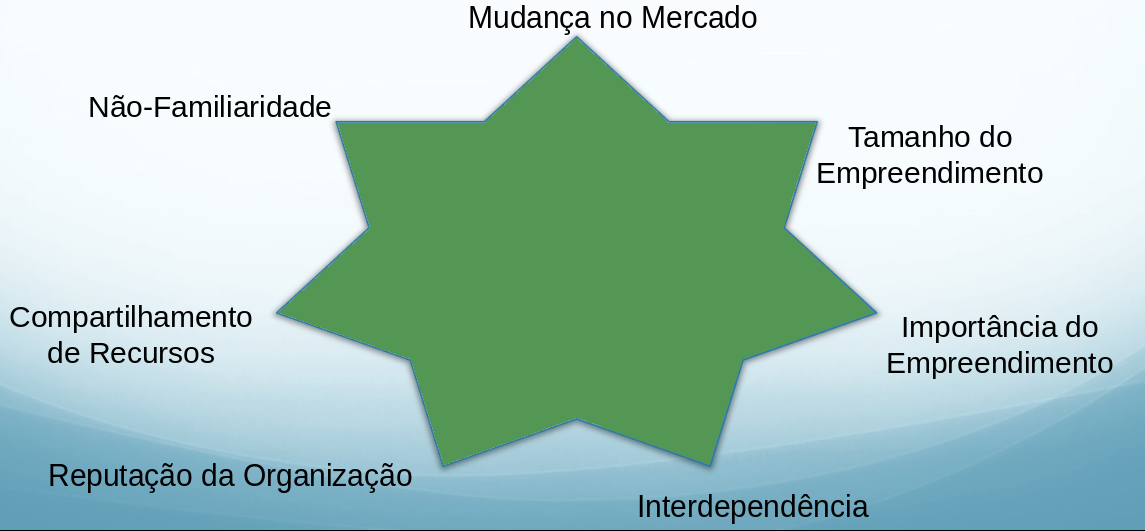
\includegraphics[width = 0.8\textwidth]{figs/fig6.png}
 \end{figure}

\end{frame}

  
  \begin{frame}
   \frametitle{Quando os Projetos são Necessários?}
   \begin{itemize}
    \item \textbf{Tamanho do Empreendimento} - Quantidade de dinheiro, pessoal e tempo superior ao normalmente aplicado
    %\pause
    \item \textbf{Interdependência} - Interdependência entre os departamentos da organização ou entre a cadeia cliente-fornecedor
    %\pause
    \item \textbf{Importância do Empreendimento} - Grande grau de risco, incerteza. Ou, minimizar burocracia organizacional	
    
   \end{itemize}
  \end{frame}
  
    \begin{frame}
   \frametitle{Quando os Projetos são Necessários?}
   \begin{itemize}
    \item \textbf{Reputação Organizacional} - Fracasso no cumprimento dos prazos e orçamentos podem prejudicar seriamente a imagem e reputação da organização
    \item \textbf{Compartilhamento de Recursos} - Reursos altamente especializado
    \item \textbf{Não-familiaridade} - Esforço é completamente novo e diferente do normal
    \item \textbf{Mudança de mercado} - Mercados extremamente turbulentos, que necessitam constantemente de atualizações
   \end{itemize}
  \end{frame}


\section{Sucesso e fracasso de Projetos}



\begin{frame}
   \frametitle{Definindo o Sucesso dos Projetos}
   \begin{itemize}
    \item Mas afinal de contas, o que é o sucesso de projetos? Segundo Kerzner:
    \begin{itemize}
     \item Na década de 60
     \begin{itemize}
      \item termos técnicos
      \item funcionamento de um produto ou serviço desenvolvido
     \end{itemize}
    %\pause
    \item Atualmente
    \begin{itemize}
     \item resultados obtidos no prazo, custo e qualidade desejados;
    \end{itemize}
    \end{itemize}
   \end{itemize}
  \end{frame}
  
   \begin{frame}
   \frametitle{Definindo o Sucesso dos Projetos}
   \begin{itemize}
    \item Ainda conforme Kerzner:
    \begin{itemize}
     \item Excelência em gerenciamento de projetos é definida como um fluxo contínuo de sucessos em projetos
    \end{itemize}
   \end{itemize}
  \end{frame}
  
     \begin{frame}
   \frametitle{Definindo o Sucesso dos Projetos}
   \begin{itemize}
    \item Detalhando os quesitos, tem-se a seguinte listagem:
    \begin{itemize}
     \item ser concluído dentro do prazo previsto
     %\pause
     \item ser concluído dentro do orçamento previsto
     %\pause
     \item ter utilizado os recursos eficientemente, sem desperdícios
     %\pause
     \item ter atingido a qualidade e o desempenho desejados
     %\pause
     \item ter sido concluído com o mínimo possível de alterações em seu escopo. (Isso vale para software?)
     %\pause
     \item ter sido aceito sem restrições pelo cliente
     %\pause
     \item não ter interrompido ou prejudicado as atividades normais da organização
     %\pause
     \item não ter agredido a cultura da organização
    \end{itemize}
   \end{itemize}
  \end{frame}
  
  \begin{frame}
 \frametitle{Fracasso de Projetos}
 \begin{itemize}
  \item Principais razões  do fracasso de Projetos
  \begin{itemize}
   \item \textbf{Pouco ou nenhum planejamento}: sem gol claro, escopo, ou timeline estabelecidos
   \item \textbf{Falta de liderança ou comprometimento dos Stakeholders}
   \item \textbf{Falta de treino} de novas tecnologias
   \item \textbf{Não há lições aprendidas} de projetos passados
   \item \textbf{Falta de treinamento} em gerencia de projeto
   \item \textbf{Viés (biases)}: otimismo, custos afundados, confirmação/inércia
  \end{itemize}
 \end{itemize}
\end{frame}

  \begin{frame}
   \frametitle{Quatro Bases para o sucesso de Projetos}
    \begin{figure}
  \centering
  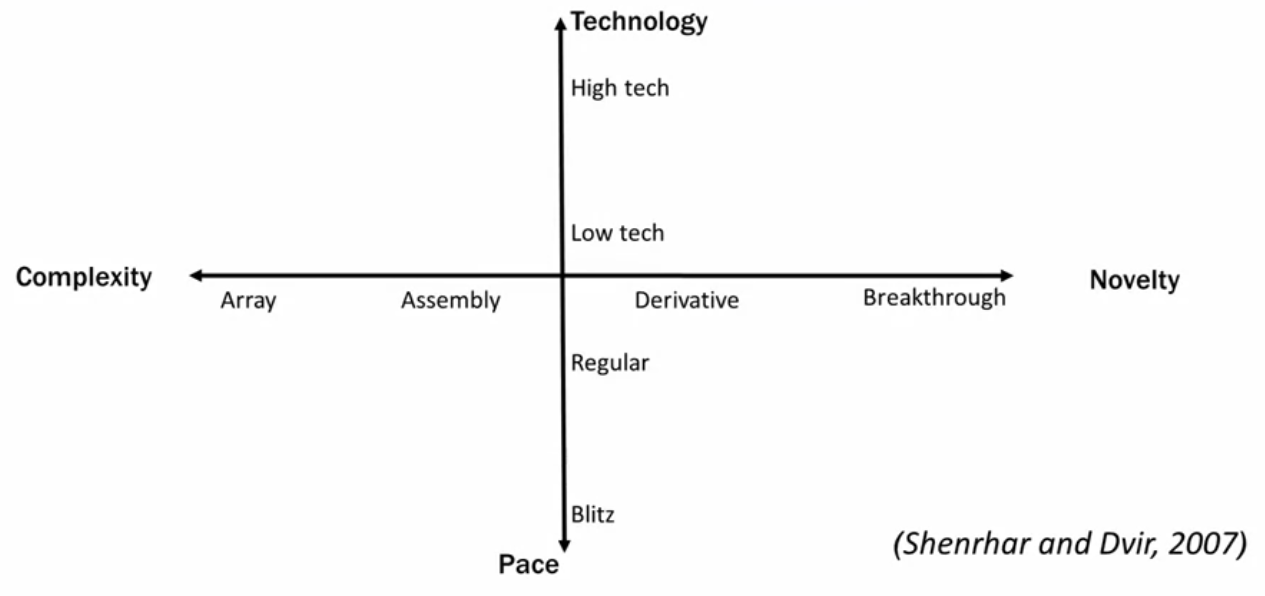
\includegraphics[width = 0.9\textwidth]{figs/fig_proj5.png}
 \end{figure}
  \end{frame}

    \begin{frame}
   \frametitle{Exemplo - Quatro Bases para o sucesso de Projetos}
   \begin{itemize}
    \item Previsão do Projeto
   \end{itemize}
    \begin{figure}
  \centering
  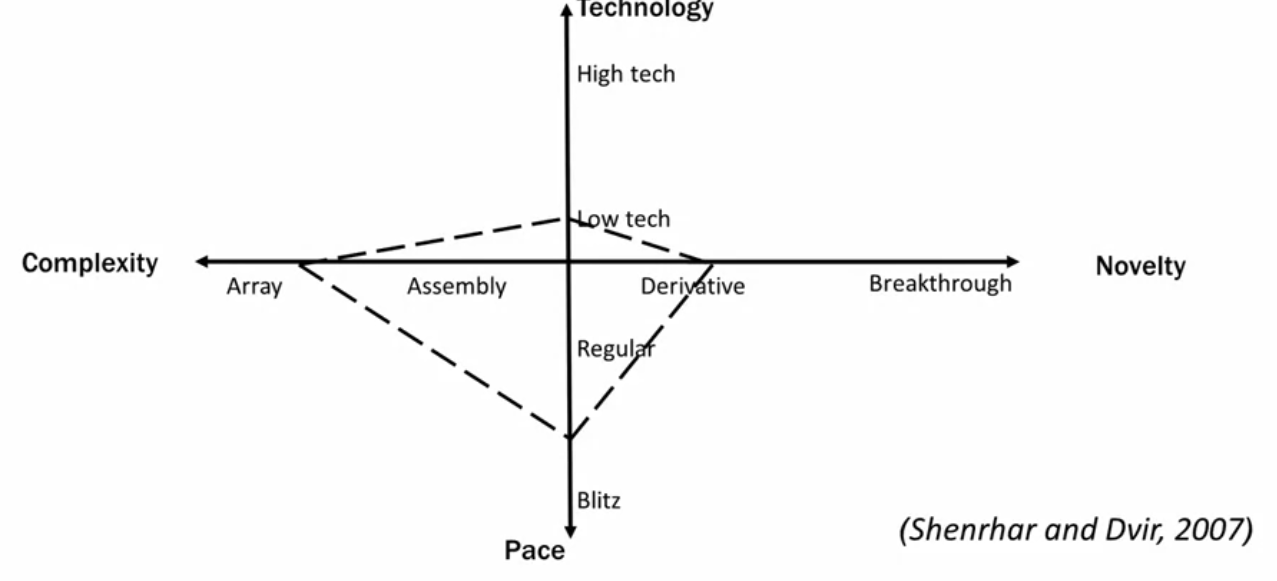
\includegraphics[width = 0.9\textwidth]{figs/fig_proj51.png}
 \end{figure}
  \end{frame}

      \begin{frame}
   \frametitle{Exemplo - Quatro Bases para o sucesso de Projetos}
   \begin{itemize}
    \item Realidade do Projeto diferente do previso - aumento da probabilidade de fracasso do projeto
   \end{itemize}
    \begin{figure}
  \centering
  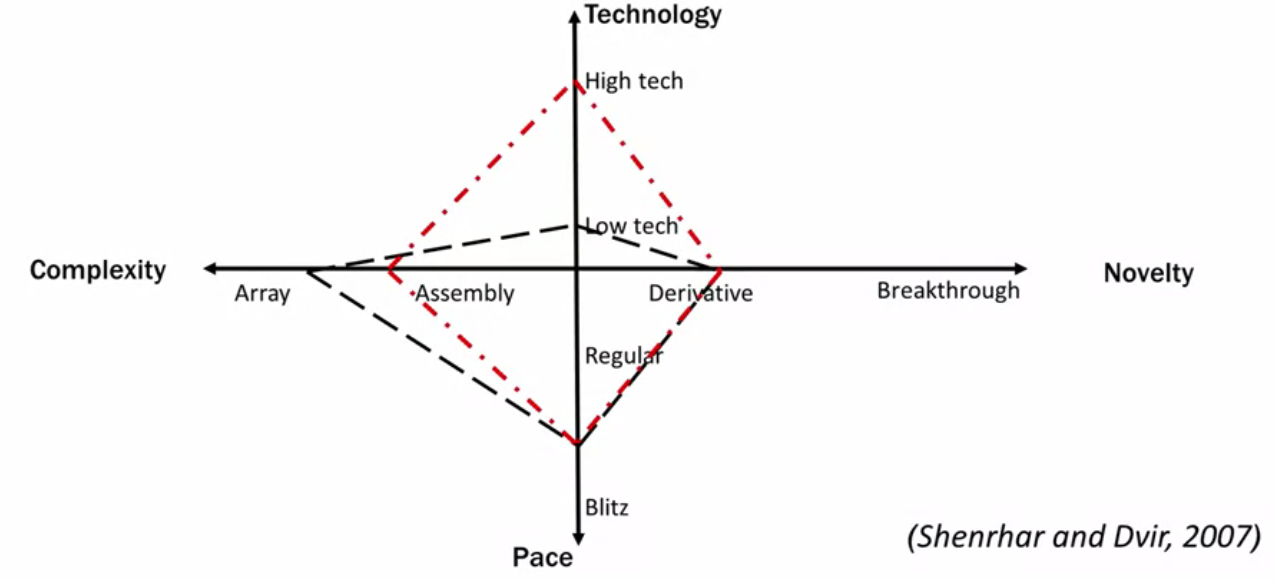
\includegraphics[width = 0.9\textwidth]{figs/fig_proj52.png}
 \end{figure}
  \end{frame}

  
  \section{Organização e Stakeholders}
  \begin{frame}
   \frametitle{Organização de Projetos e Stakeholders}
   \begin{itemize}
    \item Quem vai realizar o trabalho?
    \item Quem é o Gerente de Projeto?
    \item Quem está pagando pelo projeto?
    \item Quem vai consumir o produto ou serviço?
    \item Quem são os afetados pelo projeto?
   \end{itemize}
  \end{frame}

  \begin{frame}
   \frametitle{Stakeholders - Partes interessadas}
   Quem são as partes interessadas no projeto?
    \begin{figure}
  \centering
  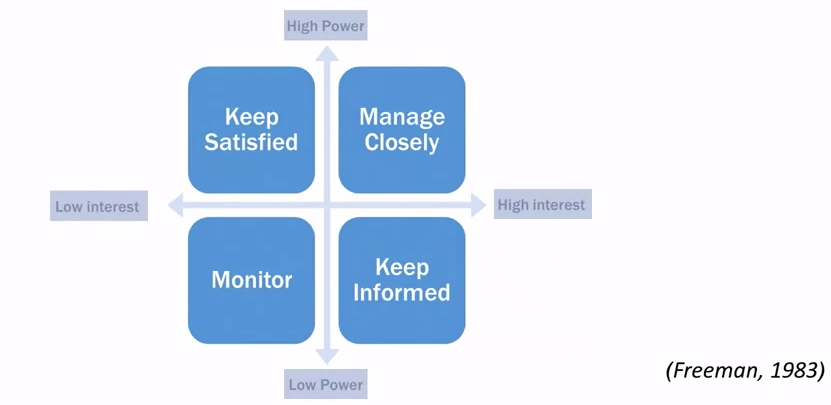
\includegraphics[width = 0.9\textwidth]{figs/fig_proj8.png}
 \end{figure}
  \end{frame}


  \begin{frame}
   \frametitle{O Gerente de Projetos}
   \begin{itemize}
    \item O gerente do projeto é a pessoa responsável pelo alcance dos objetivos do projeto
    \begin{itemize}
     \item Motivador de pessoas
     %\pause
     \item Líder do grupo
     %\pause
     \item Organizado
     %\pause
     \item Comunicador
     %\pause
     \item Influenciador
     %\pause
     \item Negociador
     %\pause
     \item Solucionador de problemas
     %\pause
     \item Gerenciador de Conflitos
     %\pause
     \item Facilitador entre processos
     %\pause
     \item Seguro nas decisões
    \end{itemize}
   \end{itemize}
  \end{frame}
  
\begin{frame}
   \frametitle{Contexto de GP
- Estruturas organizacionais}
   \begin{itemize}
    \item A organização funcional clássica é uma hierarquia em que cada funcionário possui um superior bem definido
    \begin{itemize}
     \item Os funcionários são agrupados por especialidade, como produção, marketing, engenharia e contabilidade
     %\pause
    \end{itemize}
    %\pause
    \item As organizações funcionais ainda possuem projetos, mas o escopo do projeto geralmente é restrito aos limites da função
    \begin{itemize}
     \item O departamento de engenharia em uma organização funcional fará o seu trabalho do projeto de modo independente dos departamentos de produção ou de marketing
    \end{itemize}
   \end{itemize}
  \end{frame}
  
\begin{frame}
 \frametitle{Contexto de GP - Estruturas organizacionais}
 \begin{figure}
  \centering
  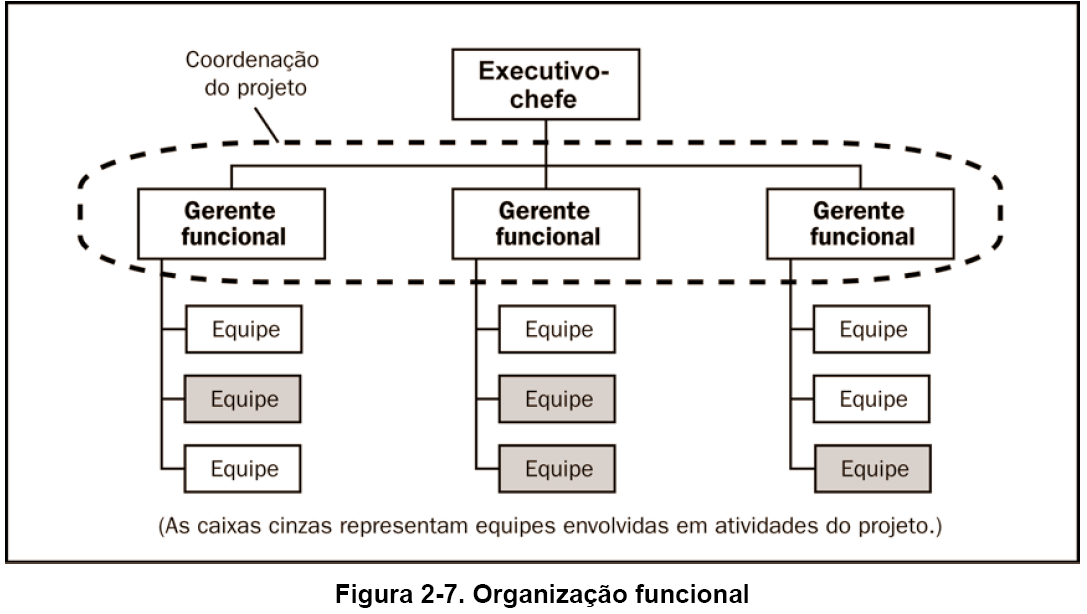
\includegraphics[width = 0.9\textwidth]{figs/fig1.png}
 \end{figure}
\end{frame}

\begin{frame}
   \frametitle{Contexto de GP
- Estruturas organizacionais}
   \begin{itemize}
    \item Em uma organização por projeto, os membros da equipe geralmente são colocados juntos
    %\pause
    \item A maior parte dos recursos da organização está envolvida no projeto e os gerentes de projetos possuem grande independência e autoridade
    %\pause
    \item As organizações por projeto em geral possuem unidades organizacionais denominadas departamentos, mas esses grupos se reportam diretamente ao gerente de projetos ou oferecem serviços de suporte para os diversos projetos
   \end{itemize}
  \end{frame}

  
  \begin{frame}
 \frametitle{Contexto de GP - Estruturas organizacionais}
 \begin{figure}
  \centering
  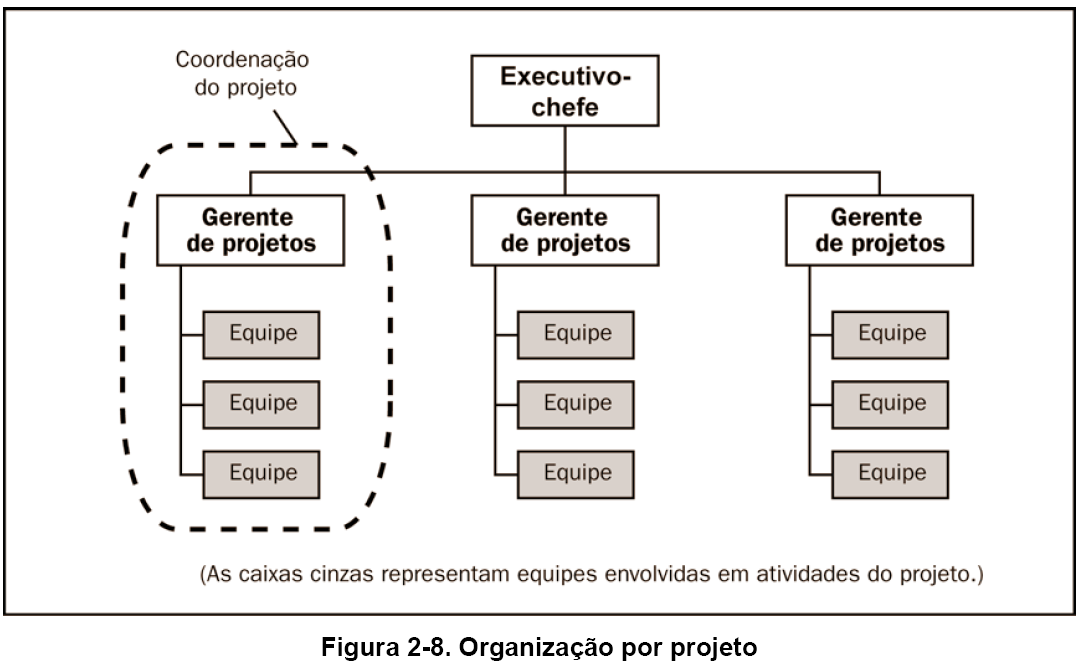
\includegraphics[width = 0.9\textwidth]{figs/fig7.png}
 \end{figure}
\end{frame}

  
  \begin{frame}
   \frametitle{Contexto de GP
- Estruturas organizacionais}
   \begin{itemize}
    \item As organizações matriciais são uma combinação de características das organizações funcional e por projeto
    %\pause
    \item As matrizes fracas mantêm muitas das características de uma organização funcional e a função do gerente de projetos é mais parecida com a de um coordenador ou facilitador que com a de um gerente
  
   \end{itemize}
  \end{frame}
  
    \begin{frame}
   \frametitle{Contexto de GP
- Estruturas organizacionais}
   \begin{itemize}
    \item Embora a organização matricial balanceada reconheça a necessidade de um gerente de projetos, ela não fornece ao gerente de projetos autoridade total sobre o projeto e os recursos financeiros do projeto
  %\pause
    \item As matrizes fortes possuem muitas das características da organização por projeto, e podem ter gerentes de projetos em tempo integral com autoridade considerável e pessoal administrativo do projeto em tempo integral. 
   \end{itemize}
  \end{frame}
  
    \begin{frame}
 \frametitle{Contexto de GP - Estruturas organizacionais}
 \begin{figure}
  \centering
  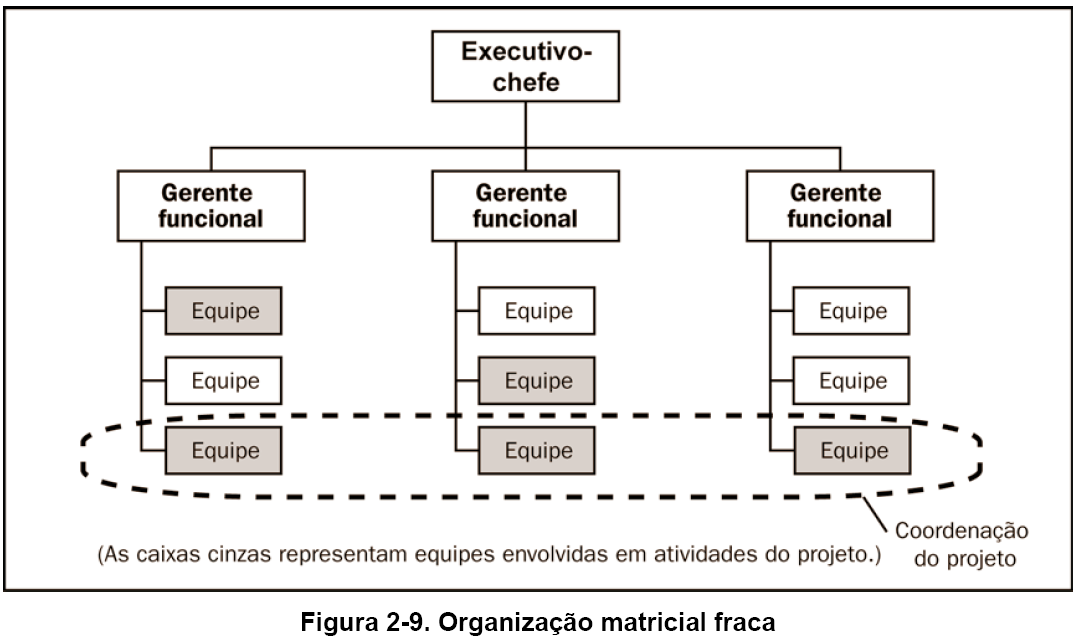
\includegraphics[width = 0.9\textwidth]{figs/fig8.png}
 \end{figure}
\end{frame}

    \begin{frame}
 \frametitle{Contexto de GP - Estruturas organizacionais}
 \begin{figure}
  \centering
  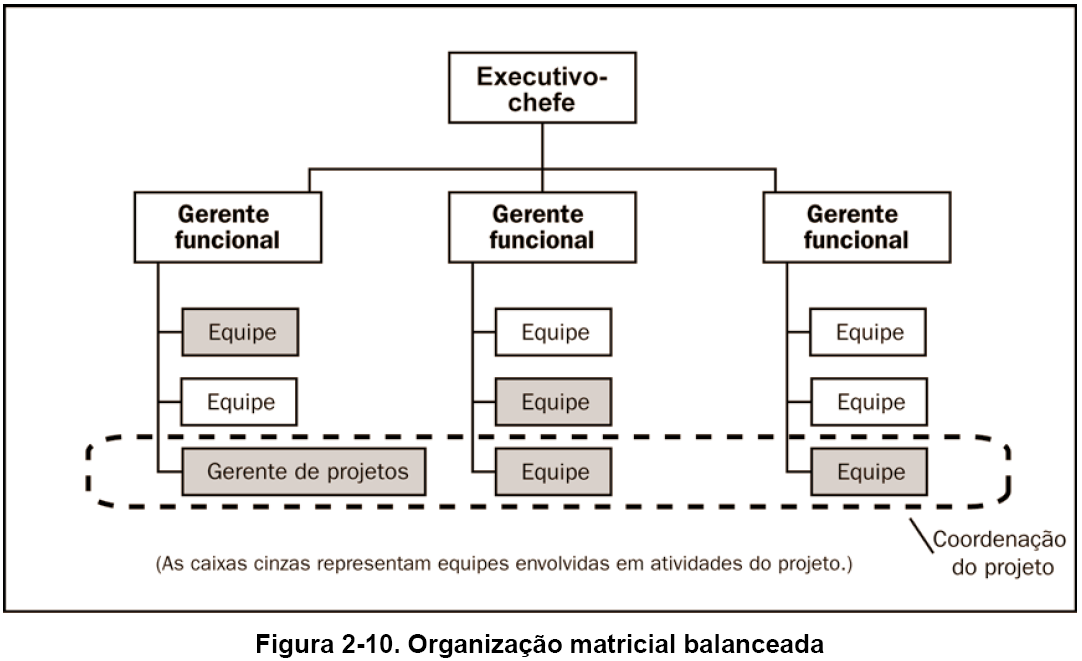
\includegraphics[width = 0.9\textwidth]{figs/fig9.png}
 \end{figure}
\end{frame}

    \begin{frame}
 \frametitle{Contexto de GP - Estruturas organizacionais}
 \begin{figure}
  \centering
  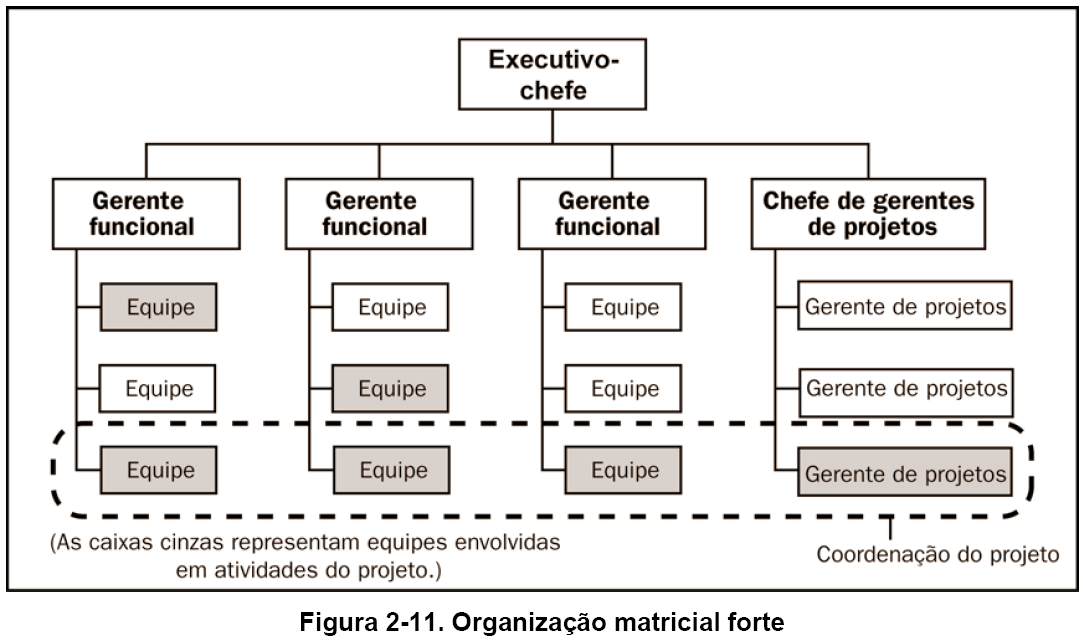
\includegraphics[width = 0.9\textwidth]{figs/fig10.png}
 \end{figure}
\end{frame}

    \begin{frame}
 \frametitle{Contexto de GP - Estruturas organizacionais}
 \begin{figure}
  \centering
  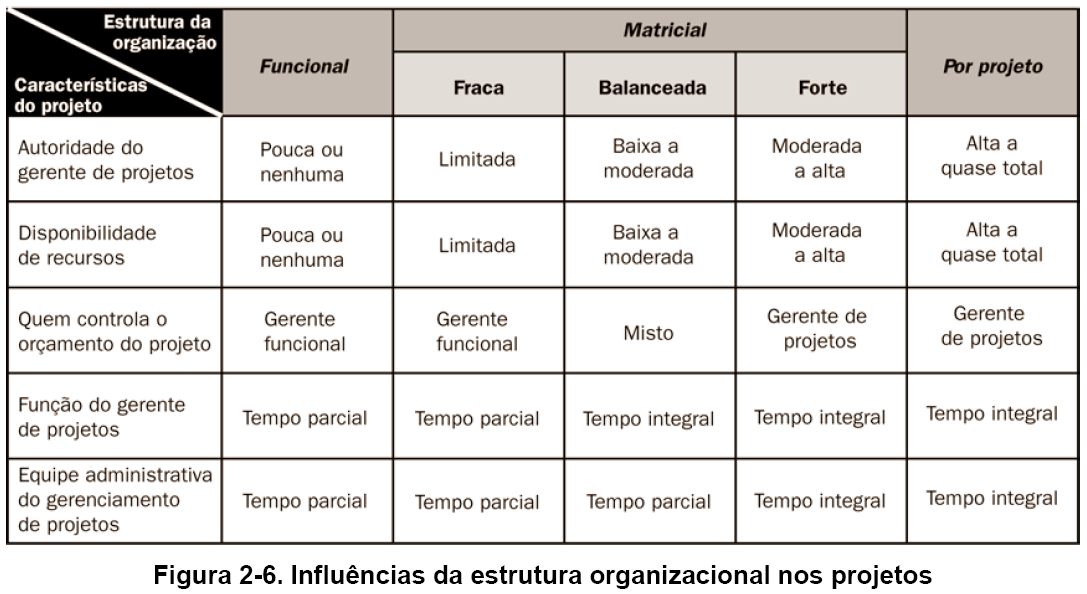
\includegraphics[width = 0.9\textwidth]{figs/fig11.png}
 \end{figure}
\end{frame}

\section{PMBok}
%     \begin{frame}
%  \frametitle{Plataforma de Gerenciamento de Projetos}
%  \begin{figure}
%   \centering
%   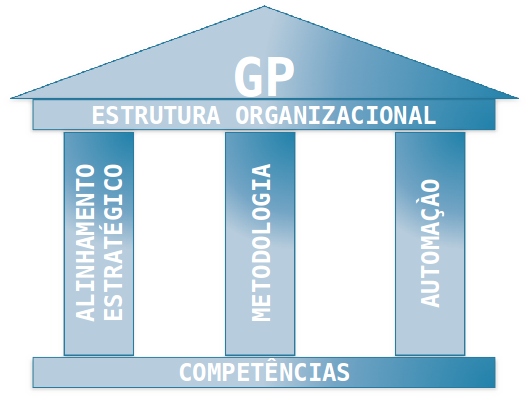
\includegraphics[width = 0.9\textwidth]{figs/fig12.png}
%  \end{figure}
% \end{frame}

  \begin{frame}
   \frametitle{O PMBoK}
   \begin{itemize}
    \item Guia para o Conjunto de Conhecimentos em Gerenciamento de Projetos – Guia  PMBOK®, que é mantido pelo Project Management Institute-PMI
    \begin{itemize}
     \item 1ª Edição em 1996
     %\pause
     \item 2ª Edição em 2000
     %\pause
     \item 3ª Edição em 2004
     %\pause
     \item 4ª Edição em 2008
        %\pause
     \item 5ª Edição em 2013
    \end{itemize}

   \end{itemize}
  \end{frame}
  
    \begin{frame}
   \frametitle{Sobre o PMBoK}
   \begin{itemize}
    \item Conjunto de conhecimentos em gerenciamento de projetos que é amplamente reconhecido como boa prática
    \begin{itemize}
     \item Visão geral, não uma descrição completa
     %\pause
     \item Conhecimento e práticas descritas são aplicáveis à maioria dos projetos na maior parte do tempo
     %\pause
     \item A aplicação correta dessas habilidades, ferramentas e técnicas podem aumentar as chances de sucesso
    \end{itemize}
    %\pause
    \item Uma boa prática não significa que o conhecimento descrito deverá ser sempre aplicado uniformemente em todos os projetos
    \begin{itemize}
     \item A equipe de gerenciamento de projetos é responsável por determinar o que é adequado para um projeto específico
    \end{itemize}
   \end{itemize}
  \end{frame} 	
  
      \begin{frame}
   \frametitle{Sobre o PMBoK}
   \begin{itemize}
    \item O conhecimento descrito no PMBOK consiste em
    \begin{itemize}
     \item Definição do ciclo de vida do projeto
     %\pause
     \item 5 grupos de processos
     %\pause
     \item 9 áreas de conhecimento
     \item 47 processos
    \end{itemize}
   \end{itemize}
  \end{frame}
  
        \begin{frame}
 \frametitle{PMBok - Áreas de  Conhecimento}
 \begin{figure}
  \centering
  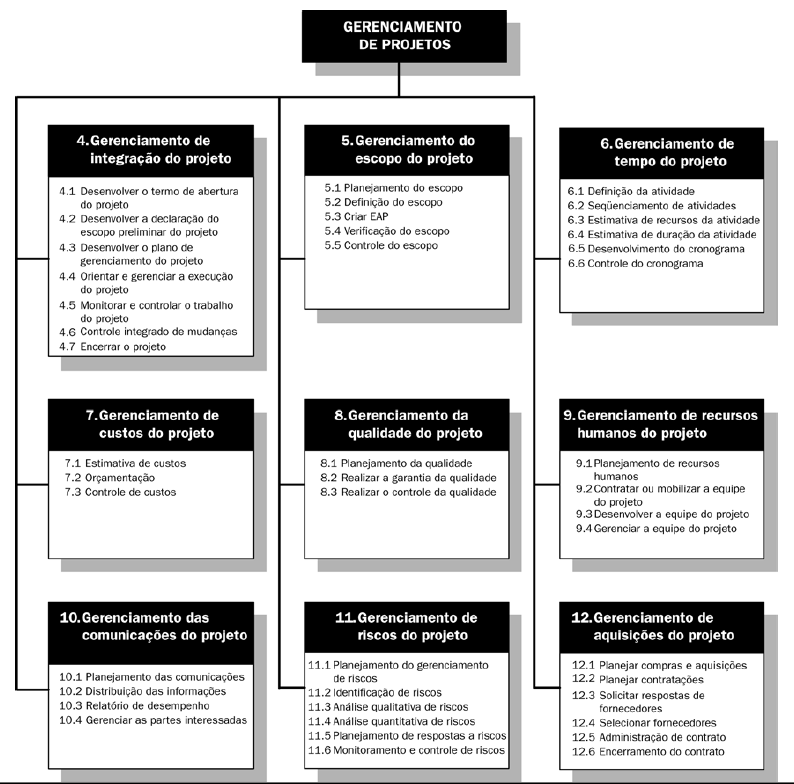
\includegraphics[height = \textheight]{figs/fig_proj7.png}
 \end{figure}
\end{frame}

      \begin{frame}
 \frametitle{PMBok - Áreas de  Conhecimento}
 \begin{figure}
  \centering
  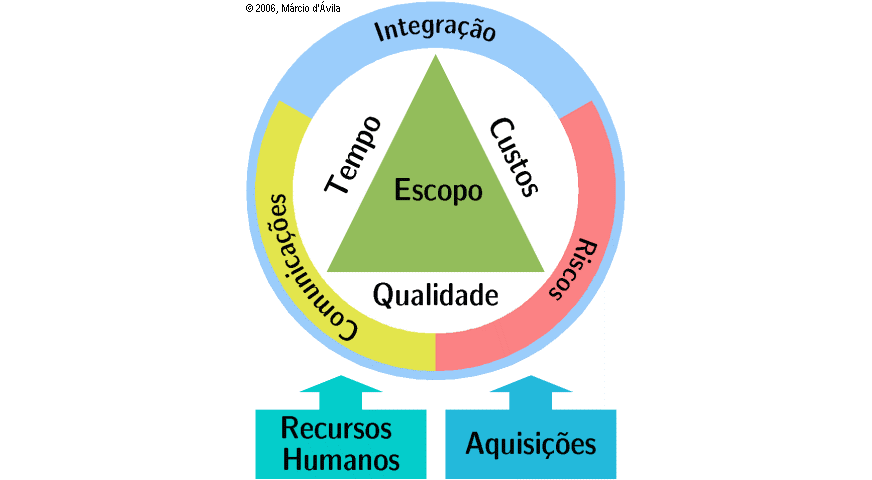
\includegraphics[width = \textwidth]{figs/fig13.png}
 \end{figure}
\end{frame}


\begin{frame}
 \frametitle{Visão Geral dos Processos de Gerenciamento de Projetos}
 \begin{figure}
  \centering
  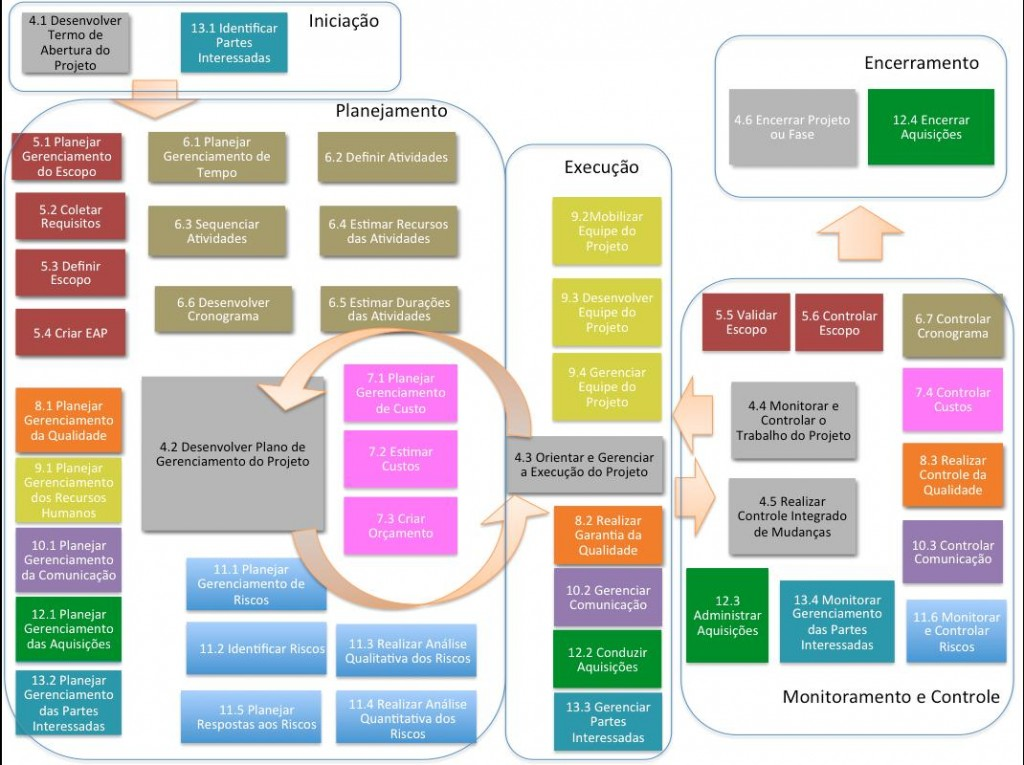
\includegraphics[width = \textwidth]{figs/figura-4-1024x765.jpg}
 \end{figure}
\end{frame}
\section{Bibliografia}
\begin{frame}
 \frametitle{Bibliografia da Aula - Leitura sugerida}
 \begin{itemize}
  \item \textit{Um guia do Conjunto de Conhecimentos em Gerenciamento de Projetos - guia PMBOK} (Cap. 1)
  \item \textit{Fundamentals of Project Planning and Management} - coursera (week 1) - \url{https://class.coursera.org/projects101-002/wiki/resources}
  \item \url{http://epocanegocios.globo.com/Inspiracao/Carreira/noticia/2015/04/12-licoes-de-tom-peters-para-ser-um-bom-lider.html}
  \item Leitura recomendada - 101 common causes of failure - \url{http://calleam.com/WTPF/?page_id=2338}
 \end{itemize}

\end{frame}

\begin{frame}
 \frametitle{Próxima Aula}
 \begin{itemize}
  \item \textit{Um guia do Conjunto de Conhecimentos em Gerenciamento de Projetos - guia PMBOK} (Cap. 2)
  \item \textit{Elaboração do Fluxo de Processos do PMBOK Guide 5ª Edição} - coursera (week 1) - \url{http://www.ricardo-vargas.com/pt/videos/1/}
  \item \textit{O perfil do Profissional do Gerente de Projetos} - \url{http://www.ricardo-vargas.com/pt/videos/7/}
 \end{itemize}

\end{frame}
